\subsection{Caratterizzazione sintetica di vettori aleatori}


\subsubsection{Media statistica}


\begin{Mybox}
    \begin{definizione}
     Si definisce \emph{media statistica} di un vettore aleatorio $\mathbf{X}$:
     \begin{equation}
        \mathbb{E}[\mathbf{X}]\triangleq
            \begin{bmatrix}
            \mathbb{E}[X_1] \\
            \vdots \\
            \mathbb{E}[X_N]
            \end{bmatrix}
        \in \mathbb{R}^N
    \end{equation}
    dove
    \begin{equation}
        \mathbb{E}[X_i]\triangleq  
        \begin{cases}
            \int_{-\infty}^{+\infty}x_ip(x_i) \,dx_i & \text{se $X_i$ è una v.a.\ continua} \\
            \sum\limits_{x_j\in\mathcal{A}_{X_i}} x_jp(x_i=x_j)   & \text{se $X_i$ è una v.a.\ discreta} 
        \end{cases} 
    \end{equation}
    \end{definizione}
\end{Mybox}


\subsubsection{Covarianza e varianza}


\begin{Mybox}
    \begin{definizione}[Covarianza]
     La \emph{covarianza} tra due vettori aleatori $\mathbf{X},\mathbf{Y}$ è così definita: 
     \begin{equation}
     \text{Cov}[\mathbf{X},\mathbf{Y}] \triangleq\mathbb{E}[(\mathbf{X}-\bm{\mu}_{\mathbf{X}})(\mathbf{Y}-\bm{\mu}_{\mathbf{Y}})^T]\label{eq:covariance}
     \end{equation}
     dove $\bm{\mu}_{\mathbf{X}}=\mathbb{E}[\mathbf{X}]$ e $\bm{\mu}_{\mathbf{Y}}=\mathbb{E}[\mathbf{Y}]$.
    \end{definizione}
\end{Mybox}

\medskip
\noindent Particolarizzando la suddetta definizione al caso in cui si consideri lo stesso vettore aleatorio $\mathbf{X}$ in entrambi gli argomenti della 
covarianza~\eqref{eq:covariance}, si ottiene la \emph{varianza} di $\mathbf{X}$.

\medskip
\begin{Mybox}
    \begin{definizione}[Varianza]
     Sia $\mathbf{X}$ un vettore aleatorio avente media $\bm{\mu}$. Si definisce \emph{varianza} di $\mathbf{X}$:
    \begin{equation}
     \begin{split}
        \mathbb{V}ar[\mathbf{X}]& = \text{Cov}[\mathbf{X},\mathbf{X}] \\
        & = \mathbb{E}[(\mathbf{X}-\bm{\mu})(\mathbf{X}-\bm{\mu})^T] \\
        & =
        \begin{bmatrix}
            \text{Cov}[X_1,X_1] &\text{Cov}[X_1,X_2] & \dots &\text{Cov}[X_1,X_N] \\
            \text{Cov}[X_2,X_1] & \text{Cov}[X_2,X_2] & \dots & \text{Cov}[X_2,X_N] \\
            \vdots & \vdots & \ddots & \vdots \\
            \text{Cov}[X_N,X_1] & \dots & \dots & \text{Cov}[X_N,X_N]
        \end{bmatrix}
     \end{split}
    \end{equation}
    \end{definizione}
\end{Mybox}

\begin{figure}
    \centering
    \subfloat[][$x$ e $y$ sono \emph{correlati negativamente}.]
   {\includegraphics[keepaspectratio]{covarianza1}} \quad
    \subfloat[][$x$ e $y$ sono \emph{correlati positivamente}.]
   {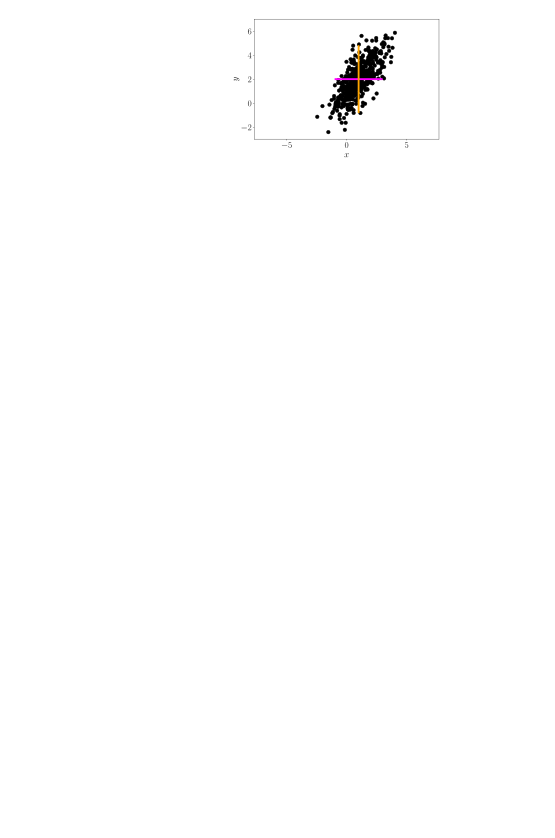
\includegraphics[keepaspectratio]{covarianza2}} 
  \caption{Due dataset bidimensionali con medie e varianze uguali (linee colorate), ma aventi covarianze diverse. Fonte~\cite{deisenrothMML2020}.}
\label{fig:bgvfcd}
\end{figure}


\subsubsection{Proprietà notevoli di media e varianza}

Siano $a, b \in \mathbb{R}$ e $\mathbf{X}, \mathbf{Y}$ due vettori aleatori. Sussistono i seguenti risultati:
\begin{align}
    \mathbb{E}[a\mathbf{X}+b\mathbf{Y}]   & = a\mathbb{E}[\mathbf{X}]+b\mathbb{E}[\mathbf{Y}] \qquad \text{Linearità della media} \label{eq:prop_media1}\\
    \mathbb{E}[a\mathbf{X}+b]   & = a\mathbb{E}[\mathbf{X}]+b \label{eq:prop_media2}\\
    \mathbb{V}ar[a\mathbf{X}+b] & = a^2\mathbb{V}ar[\mathbf{X}] \label{eq:prop_varianza1} \\
    \mathbb{V}ar[a\mathbf{X}+b\mathbf{Y}] & = a^2\mathbb{V}ar[\mathbf{X}] + b^2\mathbb{V}ar[\mathbf{Y}]+2ab\text{Cov}[\mathbf{X},\mathbf{Y}]\label{eq:prop_varianza2}
\end{align}
